%! Suppress = MissingLabel
\begin{abstract}
    
\end{abstract}

%TODO Roter Faden immer am ende des Kapitels das nächste aufgreifen
% in konzeption ruhig genauere kapitel aufgliederung
% maximal 1 seite ohne überschrift irgendeiner art


\chapter{Einleitung}
Im allgemeinen unterscheidet man bei den Gehörarten zwischen dem sogenannten absoluten Gehör und dem relativen Gehör. Während eine Person mit einem absoluten Gehör eine Note ohne eine Referenz und nur mit ihrem Gehör bestimmen kann, kann eine Person, welche nur ein ausgebildetes relatives Gehör hat, eine Note nur mit einem Vergleichston bestimmen. Wichtig ist dabei, dass die meisten Menschen das relative Gehör trainieren können, wohingegen man das absolute Gehör nicht trainierbar ist \cite{gussmack2006latentes}. Will man das relative Gehör trainieren, so hat man die Wahl aus verschiedenen Übungsansätzen und Methoden. Unter diese Methoden fallen beispielsweise das Erhören und Vervollständigen von Intervallen und Akkorden. Weiterhin werden häufig Diktate verwendet um das relative Gehör weiter zu schulen, wie etwa ein Melodiediktat, bei welchem die lernende Person die richtigen Noten einer erklingenden Melodie aufschreiben muss. \\ 
Das relative Gehör zu trainieren ist besonders wichtig für Musiker, welche zusammen musizieren, aber auch für Dirigenten, welche ihr Orchester anleiten können müssen und dabei auch potentielle Fehler ihrer Musiker erhöhren können müssen. 

\section{Motivation}
\glqq 
Study of music and
its literature presupposes the ability to hear,
read, and write the language. Lacking this ability one is
comparatively helpless and dependent. This perfectly
obvious truth is universally accepted without question
in the study of every language excepting music. Teachers, capable otherwise, allow and encourage the serious
study of music by students who do not comprehend what
they hear. Ability to hear is the essence of music, the
core of education in music is ear training
''  \cite{spencer1947ear}

Herbert S. Spencer beschreibt in einem Artikel von 1947 die Notwendigkeit der Gehörbildung um Musik in vollen Zügen wahrnehmen und ausüben zu können. Er setzt dabei das Hören von Musik mit dem Lernen von Sprachen gleich, wobei er feststellt, dass einzig in der Lehre der Musik kaum Wert auf das Hören dieser gelegt wird. Er sieht darin einen großen Verlust und beschreibt einen Musiker ohne ausgebildetes Gehör als vergleichsweise Hilflos und Abhängig. \\
Obwohl Gehörbildung bereits seit langer Zeit von Musikern als wichtig für das Musizieren wahrgenommenen wird, findet die Förderung dieser heutzutage einzig im Studium der Musik statt. Weiterhin sitzt zum Üben der Gehörbildung häufig noch ein Lehrer an einem Klavier, welcher etwas vorspielt und die Schüler ihm zuhören und das Gehörte aufschreiben müssen. Der Unterricht der Gehörbildung ist dementsprechend nicht allgemein zugänglich für die breite Masse der Musiker und stark lokalisiert in die Umgebung des Seminarsaals. Es existieren bereits einige Programme, welche bei dem Üben der Gehörbildung der lernenden Person helfen, jedoch fehlen diesen häufig die Komponente gestellte Aufgaben mithilfe von Tonerkennung automatisch zu überprüfen.
Ziel dieser Arbeit soll sein, die existierenden Trainingsprogramme zur Gehörbildung auf ihre wichtigsten Aspekte zu untersuchen und basierend auf den Ergebnissen der Analyse ein prototypisches Trainingsprogramm mithilfe von Unity3D zu entwickeln, welches die wesentlichen Aspekte der vorhandenen Software aufgreifen und verbessern soll. Das entwickelte Programm soll bestenfalls sowohl auszubildende Musiker im Studium unterstützen, als auch Amateurmusiker in der Fortbildung des Gehörs fördern. Unity bietet keinerlei Funktionen um von Haus aus eine echtzeit Tonverarbeitung zu implementieren, weshalb die Tonerkennung eine besondere Herausforderung darstellen wird. Weiterhin muss ein ansprechendes User Interface für sowohl Amateurmusiker, wie auch (auszubildende) professionelle Musiker entwickelt werden. 

\section{Aufbau der Arbeit}
Im nächsten Kapitel werden zunächst einige wichtige Definitionen zu den Oberthemen der Signalverarbeitung, Musiktheorie und zu Serious Games gegeben, welche für das restliche Verständnis der Arbeit wichtig sind. Daraufhin werden im dritten Kapitel zunächst die aktuell wichtigsten bereits vorhandenen Programme zur Gehörbildung vorgestellt und zu vorher definierten Gesichtspunkten untersucht und analysiert. Im zweiten Teil des Kapitels werden außerdem bekannte Methoden zur Tonerkennung und zur echtzeit Eingabe von Ton in Unity ebenfalls untersucht und analysiert. Basierend auf den Erkenntnissen des dritten Kapitels, wird im darauffolgenden Kapitel ein Trainingsprogramm zur Gehörbildung mit Unity konzeptioniert. Die Konzeption ist dabei aufgeteilt in 
den Entwurf des Spiels aus der Sicht des Nutzer (user-centered design), des Entwurfs der Systemkomponenten, sowie dem Evaluationskonzept. Das fünfte Kapitel beschäftigt sich anschließend mit der Implementierung des Trainingsprogramms in Unity und geht im detail auf die implementierten Funktionen ein. Das darauffolgende Kapitel beleuchtet die Evaluationsschritte näher, wobei auf die Vorbereitung und die Durchführung der Evaluation eingegangen wird, sowie die Ergebnisse der Evaluation analysiert und ausgewertet werden. Im letzten Kapitel wird schließlich eine Zusammenfassung des Themas gezogen, sowie ein Ausblick auf mögliche erweiternde Funktionen, sowie weitere Anwendungsbereiche gegeben.
%- Thema
%- Warum relevant? Wie ist es einzuordnen? (Singen macht Spaß -> Problem: Viele haben keine ausgeprägte gehörbildung, Training für Lernende)
%- Motivation: Viele haben Schwierigkeit Gehörbildung anständig zu lernen (fehlende Programme, schlechte Handhabung, festes Lernkit)
%- Allg. Fragestellung: "Viele Menschen haben Probleme..., Wollen Lernen..., Müssen im Rahmen ihres Studiums lernen..."
%- techn. Problemstellung: "Realtime Soundverarbeitung unter UNity mit angemessener Fehlerquote / Intuitives Design der Notenausgabe/Platzierung auf das Notensystem"
%Introkapitel
%- Thema beschreiben 
%- Problemstellung grob eingehen
%-- facettenreiche und betrifft die folgenden gebiete
%--- serious games, audio, Grundlagen..
%y-- als nächstes schau ich das näher an -> rundown der arbeit geben



\chapter{Grundlagen}
\section{Signalverarbeitung}
%- Frequenz
%- Abtasttheorem
%- FFT
%- Unity eingebauten Methoden
\subsection*{Nyquist-Shannon-Abtasttheorem}
\label{sec:Abtast}
Das Nyquist-Shannon-Abtasttheorem besagt, dass eine Frequenz $f_{max}$ nur dann exakt rekonstruiert werden kann, wenn es mit einer mindestens doppelt so hohen Frequenz $2f_{max}$ abgetastet wird. Auf die Akustik bezogen heißt das also, dass man um eine Frequenz von 20kHz ohne Verlust aufzunehmen, 
man den Ton mit mindestens 40kHz abtasten muss.

\subsection*{Fouriertransformation}
\label{sec:Fouriertransformation}
Eine Fouriertransformation ist eine Methode, mit der man ein Signal in ein Spektrum zerlegen kann. Diese Definition ist bewusst weitläufig gewählt, da ich nun nur auf die relevante spezifischere Bedeutung, im Zusammenhang mit Akustik, eingehen werde.
Da sich bei einem Ton ein bestimmtes Muster über einen endlichen Zeitraum wiederholt, handelt es sich um ein periodisches Signal. Es wird also eine Fouriertransformation angewandt, welche ein
periodisches Signal in ein Linearspektrum zerlegt. Ein Signal zu zerlegen heißt dabei nichts anderes, als mit einer endlichen Summe an Sinusschwingungen zu modellieren. Untersucht man die entstandene Funktion, so kann man die im Signal vorhandenen Frequenzen 
herausfiltern bzw. erkennen. Diese Eigenschaft ist offensichtlich essenziell bei der Tonerkennung. Es treten Probleme auf, falls eine nicht ganzzahlige Anzahl an Perioden untersucht wird, was so viel heißt, dass eine Periode abgeschnitten wurde. Es kann dann zu \glqq schwammigen'' Spektren kommen.
Dieses Problem kann durch Fensterfunktionen beseitigt werden. Fensterfunktionen sorgen dafür, dass die Amplituden an den Flanken weich gezeichnet werden, sodass die Endpunkte der Perioden aneinander angeglichen werden und es zu keinen unstetigen Übergängen kommt \cite{Butz2006}.

\section{Musiktheorie}
\subsection*{Intervalle}
\label{sec:Intervalle}
Ein Intervall im musikalischen Sinn bezeichnet den Tonabstand zwischen zwei Tönen. Man kann dabei zwischen den sogenannten harmonischen Intervallen und den melodischen Intervallen unterscheiden. Bei den harmonischen Intervallen erklingen die Töne
gleichzeitig, wohingegen bei melodischen Intervallen die Töne hintereinander erklingen. Intervalle lassen sich mathematisch als Proportionen der erklingenden Töne zueinander beschreiben, das wichtigste Intervall ist hierbei die Oktave. Die Oktave hat ein Frequenzverhältnis von 2:1, 
sie entspricht also immer der doppelten Frequenz von einem Ton zu dem anderen und kann von mehreren Tonsystemen unterteilt werden. Alle dieser Unterteilungen benennen die Schritte innerhalb einer 
Oktave nach den lateinischen Ordinalzahlen, wobei Oktave Acht bedeutet. Wie der Name Oktave also schon vermuten lässt, liegen innerhalb einer Oktave sieben andere Intervalle. Diese Annahme ist allerdings nur bedingt richtig, da neben den sieben nach den Ordinalzahlen benannten Intervallen, auch 
große und kleine, sowie verminderte und übermäßige Intervalle existieren. Diese weitere Einstufung der Intervalle ermöglicht es Intervalle mit einem halben Ton abstand zu notieren, neben den Ganztönen. Berücksichtigt man all das, so lässt sich eine Oktave in 
12 Halbtöne aufteilen, wobei jeder mögliche Abstand zwischen diesen Halbtönen benannt werden kann. \\\\
Es gibt neben den Einteilungen von Intervallen innerhalb einer Oktave auch bezeichnungen für Intervalle, welche einen Abstand größer als eine Oktave umspannen. Ich möchte diese aufgrund der Vollständigkeit auch erwähnen, jedoch werden diese nicht weiter in der folgenden Arbeit berücksichtigt.
Diese Intervalle folgen weiterhin der lateinischen Ordinalzahlreihe, sodass ein Intervall, welches einen Ganzton weiter umspannt als die Oktave, dementsprechend None genannt wird. \cite{abcmusik}

\subsection*{Die Grundfrequenz und Obertöne}
\label{sec:Oberton} \label{sec:Nebenschwingung} \label{sec:Grundfrequenz}
Bei allen musikalisch erzeugten Tönen treten neben dem sogenannten Grundton bzw. der Grundfrequenz auch Nebenschwingungen oder Obertöne mit auf.
Bei der Grundfrequenz handelt es sich um die tiefste auftretende Schwingung in diesem Spektrum, die restlichen messbaren Schwingungen sind die sogenannten Obertöne, diese bestimmen vorallem die Klangfarbe, verändern aber nicht den erklingenden Ton in seiner Höhe.
In der Musik bestimmt also die Grundfrequenz den wahrgenommenen erklingenden Ton und die Obertöne nur die Wahrnehmung des Tons. Die Obertöne können dabei aber häufig einen stärkeren Ausschlag verursachen, untersucht man einen Ton mithilfe
einer Fouriertransformation. Ein Ton im musikalischen Sinn beschreibt also nicht eine reine Sinuswelle, sondern vielmehr eine überlagerung mehrerer Schwingungen, welche zusammen den Ton mit Klangfarbe ausmachen. Obertöne sind in der Regel ganzzahlige vielfache 
des Grundtons, Töne mit dieser Eigenschaft nennt man Harmonisch. Ausnahmen zu dieser Regel sind vorallem Klänge welche für das menschliche Ohr als unschön oder störend empfunden werden, wie
beispielsweise Glocken oder fallende Rohre und Stangen, sie werden auch unharmonisch genannt. \cite{abcmusik} \cite{harmonische_obertne}


\subsection*{Tonsysteme und Stimmung}
\label{sec:Tonsysteme}
Wie bereits in \ref{sec:Intervalle} angesprochen, gibt es verschiedene Systeme um die Tonabstände zu bestimmen, ich möchte hier nun die wichtigsten dieser Arten beleuchten und auf ihre Anwendungen und Herkünfte eingehen.
Verschiedene Arten von Unterteilungen werden auch Stimmungen genannt. Betrachten wir zunächst den Tonraum, in welchem wir un befinden. \\
In dem geordneten Tonraum lässt sich jedem Ton genau eine Frequenz zuordnen, wobei gilt, umso höher die Frequenz, desto höher ist auch der erklingende Ton. Außerdem ist jedem Paar von Tönen $t_1, t_2$ bzw. Frequenzen $f_1, f_2$ genau ein Intervall $i_{12}$ zugeordnet, 
wir können daraus folgern, dass das Intervall der Töne, ein Frequenzverhältnis von $f_2 : f_1$ hat. Es wird außerdem in der Musik die Einheit Cent herangezogen um genauere Angaben zu verschieden hohen Tönen zu machen. Ein Cent ist definiert als 
$1/1200$ Oktave. Betrachtet man den Raum der Intervalle und der Frequenzverhältnisse, so fällt auf, dass ein Homomorphismus zwischen diesen beiden Räumen gegeben ist. Addiert man zwei Intervalle im Intervallraum, so multipliziert man deren Frequenzverhältnisse bzw. Proportionen. \\
Ein kurzes Beispiel soll diesen Zusammenhang verdeutlichen. Nehmen wir die kleine Terz $i_1 =  316$ Cent und die Quinte $i_2 =  701$ Cent und ihre dazugehörigen Frequenzverhältnisse $p_1 = 6/5$ und $p_2 = 3/2$ als gegeben an.
$$    i = i_1 + i_2 = 1017  $$
$$    p = p_1 * p_2 = 9/5   $$
$$   => 1200 * \log_2{9/5} \approx 1017     $$
\\
Es gibt nun verschiedene Verhältnisse welche verschiedene sogenannte Stimmungen bilden. Zu den bekanntesten Stimmungen zählen die reine Stimmung, die pythagoreische Stimmung und die gleichstufige Stimmung.
All diese Stimmungen haben die Gemeinsamkeit, dass sie durch Cent beschrieben werden und somit alle eine Oktave als 1200 Cent bzw. als ein Stimmungsverhältnis von 1:2 definieren. Die Unterschiede der Stimmungen ergeben sich dann, wie die einzelnen
Töne gestuft sind. Die älteste Stimmung aus dem europäischen Raum ist die pythagoreische Stimmung. Pythagoras reihte für die Berechnung zwölf Quinten aneinander und erhielt so sieben Oktaven höher wieder den Ausgangston. Bei dieser Stimmung traten einige 
ungereimtheiten auf, sodass bspw. das fis einige Cent höher lag als das ges. Dieser Unterschied wird das pythagoreische Komma genannt. Die Töne fis und ges wurden später von der gleichstufigen Stimmung gleichgesetzt. Die gleichstufige Stimmung definiert einen Halbtonschritt als 100 Cent, sodass die ganze Oktave gleichstufig verteilt ist und das
pythagoreische Komma aufgelöst wird. Die reine Stimmung basiert, entgegen der anderen beiden Stimmungen, auf der natürlich auftretenden harmonischen Obertöne (\ref{sec:Oberton}) eines Tons. Bei der reinen Stimmung treten noch mehr Probleme mit der Bestimmung der Ganz und Halbtonschritte auf. Es ergeben sich aus der Definition der reinen Stimmung zwei verschiedene Frequenzverhältnisse für einen Ganzton. \cite{abcmusik}

\section{Serious Games}
Serious Games sind digitale Spiele, welche nicht nur unterhalten sollen, sondern auch ein weiteres Ziel verfolgen. Dies wird gemacht, um eine Brücke zwischen Bildung und der Vermittlung von neuem Wissen und Unterhaltung zu schlagen. Dieses Ziel wird auch das Characterizing Goal genannt. Dabei ist es wichtig, dass Serious Games dieses zusätzliche Ziel umsetzen wollen, ohne dabei den Spielspaß oder die generelle Spielerfahrung einzuschränken. Die Spiele sollen weiterhin das Hauptziel der Unterhaltung verfolgen. Einige prominente Beispiele sind Spiele, wie etwa \glqq Coding Pirates'' \cite{coding_game}, welches neues Wissen vermitteln möchte, oder ein Spiel welches zur Bewegung anregen möchte, wie etwa \glqq Pokemon Go''\cite{althoff2016influence} oder die \glqq Moto Tiles'' \cite{liu2018playful}. Um Serious Games einheitlich klassifizieren zu können, wurde das sogenannte \glqq Serious Games Metadata Format'' entwickelt. Dieses Format ist aufgebaut aus mehreren Stufen. Die erste Ebene (Core), enthält allgemeine Informationen über das Spiel, welche Interessenten einen Überblick über die Qualität, Innovationen und Anwendungen des Spiel geben sollen. Die zweite Ebene (Detailed) dient Kritikern und Experten als Grundlage der Bewertung eines Serious Games. Sie beinhaltet daher Punkte wie etwa Informationen zur User Experience und einem Fragebogen zur generellen Bewertung. Auf der dritten Ebene (Extension) wird schließlich eingegangen auf spezifische Aspekte des Spiels eingegangen. So werden hier beispielsweise bei Exergames Trainingsprogramme und genaue Sportübungen bewertet \cite{gobel2011makes}. Eine Plattform um nach dem Metadaten Format Spiele zu filtern ist das Serious Games Information Center (SG-IC) \cite{sg_ic}. \\
Im Gegensatz zu einem Serious Game steht das Konzept der Gamification. Bei der Gamification handelt es sich um den Ansatz spielerische Komponenten in eine Umgebung einzubinden, welche kein Spiel ist. Populäre Beispiele für Anwendungen, welche Gamification umsetzen, sind \glqq Duolingo'' \cite{duolingo}. Spielerische Elemente können ein Highscore System mit online Leaderboard sein oder die Möglichkeit Trophäen zu sammeln. Die Gamification Elemente sollen dem Nutzer meistens ein Gefühl von Fortschritt geben. 
% TODO add Serious Games kapitel, ganz grob beschreiben

\chapter{Analyse}

%- Wie in der Rechereche vorgegangen (Kontakte, Anhaltspunkte, Wissenschaftler, Suchbegriffe, wichtigste Filter) -> Top Referenzen
%- Studentin befragt nach bestem SotA
%- Was fehlt, was könnte besser sein?
%- Hobby Musiker befragt ob sie soetwas kennen und Interesse hätten, wie wäre es Interessant?
%- Gehörbildungslehrer / Musiklehrer befragen, woran es häufig hakelt und was interessant ist in so einem Programm
%
%
%- tech. Knackpunkt: Wie macht die Game Engine etwas? (Sound Verarbeitung etc.)
%- Auslesen der Mikrofon Daten und direkte Umrechnung mithilfe von gegebenen FFT Methoden in Unity
%- PDA im Rahmen dieser Möglichkeiten
%- Warum keinen komplexeren PDA implementiert ohne eingebaute Unity FFT
Im folgenden Kapitel werde ich zunächst auf den aktuellen Stand der Trainingsprogramme für Gehörbildung eingehen und diese auf ihre wichtigsten Aspekte analysieren und wie man diese noch verbessern könnte. Daraufhin werde ich nach Methoden und Konzepten zur Echtzeiterkennung von Audio mit Unity recherchieren und analysieren, um diese in einen Prototypen eines Trainingsprogramms einzubinden.

\section{Analyse von Trainingsprogrammen zur Gehörbildung}
%- auf bestimmte Aspekte achten, bei der Analyse
%    - Audio Input?
%    - Arten von Übungen 
%        - Vielfalt
%        - Abdeckung der musikalischen Bereiche (Intervalle, Akkorde, )
%    - Übungsvielfalt
%        - festes Set oder Endlosübungen
%    - Navigierbarkeit
%    -Pädagogisches Konzept
Ich stelle zunächst die bekanntesten Anwendungen und Websites zum Training der Gehörbildung vor.
\subsection{Methodik}
%TODO Methodik
%- Auf Pitch Detection achten
%- Übungsarten x 
%- Einführung in Thema  (theorieteil) x
%- Wieder(spielbarkeit) x
%
%- Audio Input?
%    - Arten von Übungen 
%        - Abdeckung der musikalischen Bereiche (Intervalle, Akkorde, )    x
%    - Übungsvielfalt x
%        - festes Set oder Endlosübungen x
%    - Navigierbarkeit x
%    -Pädagogisches Konzept x

% Übung
Ich werde bei der Begutachtung der State of the Art Anwendungen vorallem auf die Aspekte der Übungsvielfalt, sowie dem Aufbau der Übungen achten. Unter die Übungsvielfalt fällt unter anderem eine Einschätzung der Wiederspielbarkeit und des abgefragten Wissens, sowie die Breite der verfügbaren Übungen zu verschiedenen musikalischen Bereichen innerhalb der Gehörbildung. Zu diesen Bereichen zählen beispielsweise Intervalle, Akkorde, oder Melodiediktate.
% Pädagogisches Konzept
Außerdem möchte ich auf die Weiterbildungsmöglichkeiten und die generelle Wissensvermittlung achten. Unter Wissensvermittlung verstehe ich hier, ob das Wissen beispielsweise innerhalb des Spiels vermittelt wird, oder nur zum Nachlesen bereitsgestellt wird. 
% Input + UI
Weiterhin interessiert mich wie der Nutzer mit der Anwendung interargieren kann, dabei sind die Punkte der Navigierbarkeit, die Eingabemöglichkeiten, sowie der generelle Aufbau des UIs wichtig. 

\subsection{State of the Art}

Zu den State of the Art Programmen gehören vorallem online Tools zur Unterstützung bei der Gehörbildung. Die folgenden Tools habe ich vorallem durch Befragung von Musikstudenten, sowie durch einfach Suchanfragen gefunden.

\subsection*{Gehörbildungswebsite der staatlichen Hochschule für Musik und darstellende Kunst Mannheim}
\label{sec:Mannheim}
Hierbei handelt es sich um ein online Tool, bei welchem aus einer festen Anzahl an aufgenommen Hörbeispielen Übungen generiert werden.
Dabei werden die Themen Intervall- und Akkord-Intonation, sowie eine Möglichkeit zur Überprüfung der eigenen Fähigkeiten angeboten. Das Intervalllernen ist so strukturiert, dass der Nutzer Töne vorgegeben bekommt
und die Intervalle zwischen den Tönen bzw. zu einem Grundton bestimmen soll. Die Website überprüft dabei nicht selbst, ob der Nutzer die Aufgabe richtig absolviert hat, der Nutzer muss sich selbst überprüfen. 
Es gibt mehrere Arten von Intervalltraining, so kann man seine Fähigkeiten in diatonischen Stufen, also innerhalb einer Tonleiter ohne Halbtöne, oder reines Intervalle erkennen zwischen einzelnen Tönen, verbessern. Es gibt weiterhin die Möglichkeit in ganzen Tonreihen
direkte und indirekt erklingende Intervalle zu erhören bzw. Wahrzunehmen. Außerdem bietet die Website vorgefertigte Übungen zu Rhythmus, Melodie, Akkorden, Harmonik und Intonation an. Man erhält zugriff auf die Übungen, nachdem man einen Account 
erstellt hat. Die Übungen sind dann unterteilt in einzelne Reiter in die einzelnen Lektionen. Es existiert ein kurzer einleitender Text, welcher den Nutzen der Website kurz erläutert und eine schnelle ERklärung, wie vorzugehen ist beim Lernen. Es werden keine 
Module oder Lektionen angeboten, welche die Grundlagen der Aufgaben näher erläutern.\\
Die Website bietet allerdings nur die Aufgaben an, das heißt es gibt keine eingebaute Überprüfung, weder als Texteingabe noch als Audioinput vom Nutzer. \cite{hfmdk_mannheim}

\subsection*{Musictheory.net und Tenuto}
\label{sec:Musictheory.net} \label{sec:Tenuto}
Die Website Musictheory bietet eine vielzahl von Übungen in verschiedenen Disziplinen an. Es existieren theoretische Lektionen, welche das fundamentale Wissen herstellen sollen, sowie Übungen, um dieses abzufragen und zu testen. 
Die Lektionen umfassen die Grundlagen der Musik, wie etwa die verschiedenen Notenschlüssel oder das Notenlesen, bis hin zu verschiedenen Arten von Akkorden und wie diese aufgebaut werden. Die Übungen umfassen dementsprechend ein ähnlichen 
Wissensumfang, es wird beispielsweise das Notenlesen abgefragt oder die Tonart, aber man kann auch Gehörbildung üben, wo man das Erkennen von Tönen bis hin zu Akkorden üben kann. Bei diesen Übungen kann man
allerdings nur das gehörte aus einer List auswählen. Ein Unterschied zu der Website der HfMdK Mannheim besteht darin, dass Musictheory.net Antwortmöglichkeiten gibt und bei diesen ein Feedback gibt, ob 
die Antwort richtig war. Auch hier gibt es kein Features, welches gesungene Intervalle überprüft. Musictheory.net hat eine App für iOS entwickelt, welche die Aufgaben, welche auch auf der Website zur Verfügung stehen,
mit erweiterten Funktionen bereitstellt. Die Funktionen der App umfassen zusätzlich zu den Aufgaben der Website eine Möglichkeit Aufgabetypen anzupassen umso Aufgabentypen spezifisch zu lernen. Desweiteren wurde ein Challenge Modus in der 
App hinzugefügt, welcher den Nutzer herausfordert unter Zeitdruck Aufgaben richtig zu beantwortern und den Highscore zu verbessern. Das User Interface der App wird extra beworben auf der Website als einfach zu bedienen und mit einer klaren Benutzer Erfahrung. 
Die App kostet 3.99\$, wohingegen die Website kostenfrei ist und ohne Benutzeraccount verwendet werden kann. Es ist noch anzumerken, dass sowohl die Website, als auch die App nur auf Englisch verfügbar sind, was eine Behinderung für den Nutzer darstellen kann. \cite{musictheory}

\subsection*{Teoria}
\label{sec:Teoria}
Teoria bietet ähnlich wie Musictheory, einen Theorieteil und einen Praxisteil an. Im Theorieteil werden auch hier die Grundlagen der Musik vermittelt, wie beispielsweise das Notenlesen oder was ein Intervall ist und wie diese aufgebaut werden.
Im praktischen Teil ermöglicht Teoria es dem Nutzer seine eigenen Aufgaben selbst zu gestalten, indem man die abzufragenden Intervalle einstellen kann oder auch den Grundton. Es ist außerdem möglich das sogenannte vom Blatt Singen zu trainieren, was nichts anderes
heißt als direkt die Noten und den Rhythmus richtig zu singen, ohne es vorher gehört oder geübt zu haben. Das Singen wird allerdings auch hier nicht überprüft, es ist nur ein Angebot gegeben sich selbst überprüfen zu können. Es werden weiterhin Übungsangebote in den
Aufgabenbereichen der Intervalle, Akkorde, des Rhythmus und der Tonarterkennung. Die Aufgaben werden durch den Nutzer voreingestellte Parameter zufällig generiert und können somit auch an die Bedürfnisse des Nutzer angepasst werden. 
Die Website hat ein relativ einfaches und intuitives Design, ist allerdings nur auf Englisch verfügbar, was beispielsweise die Namen der Akkorde betrifft und durchaus eine Umstellung für den Nutzer darstellen kann. \cite{teoria}

\subsection*{JKG Neigungskurs Musik}
\label{sec:Neigungskurs}
Die Website des Justus-Knecht-Gymnasium Bruchsaal bietet ein kleines vordefiniertes Set an Aufgaben, für die Vorbereitung auf die Musik Abiturprüfung, an. Zu den Aufgabentypen zählen Rhythmusdiktate, Melodiediktate, sowie Intervalle und Akkorde erkennen.
Wie bereits erwähnt sind die Aufgaben vordefiniert und bieten keinerlei Möglichkeit sie anzupassen nach den Bedürfnissen des Nutzers. Die Aufgaben bilden eine grobe Übersicht über die möglichen Aufgabentypen und dienen nur als Lernhilfe oder zur Überprüfung, sind jedoch 
nicht geeignet als alleiniges Lernmittel oder zur täglichen Festigung der Fähigkeiten. Es existiert dementsprechend auch keine Schrittweise Einführung in die Grundlagen der Musik oder der Gehörbildung. Desweiteren ist die Bedienbarkeit und Nutzerfreundlichkeit auf der mangelhaft, da die Soundbeispiele über Soundcloud zwar in die Website eingebunden sind, jedoch die Lösungen nur in 
PDFs zu finden sind, welche zunächst heruntergeladen werden müssen. \cite{jkg_bruch}

\subsection*{Musikgrad}
\label{sec:Musikgrad}
Musikgrad bietet einige simple Aufgabentypen und Trainingsmethoden zu Intervallbestimmung, aber auch zu der Bestimmung von Akkorden und den Grundlagen der Musik, wie etwa das Notenlesen. Die Theorieaufgaben bzw. Lektionen sind dabei strukturiert in Lektionen und Module innerhalb einer Lektion, welche das Thema so Schritt für Schritt näher erläutern. Da einige Aufgaben allerdings leider Flash Player benötigen, sind diese nicht mehr
zugänglich. Ich beschränke mich im Folgenden nur auf die verfügbaren Aufgaben, welche allerdings immernoch die wichtigsten Funktionen abdecken. Es wird die Möglichkeit geboten Intervalle zu erhören, dabei werden zwei Töne gleichzeitig abgespielt und der Nutzer muss aus allen Intervallen
entscheiden, welches erklungen ist. Es wird dabei die Möglichkeit gegeben, die abzufragenden Intervalle zu konfigurieren, umso auf eigene Schwächen genauer einzugehen. Es gab offensichtlich mal die Möglichkeit auch zu einem gegebenem Grundton ein Intervall zu vervollständigen in einem Notensystem, diese Funktion
ist allerdings mittlerweile veraltet und nicht mehr Verfügbar. Auch bei Musikgrad gibt es keine Möglichkeit, dass der Nutzer singen kann und dieser Gesang automatisch überprüft und angezeigt wird. Die Website an sich ist simpel aufgebaut, sodass man durch eine einfache Auswahl zu den verschiedenen Übungen kommt. Die Übungen sind
verfügbar innerhalb einer eingebundenen Anwendung im Browser, sodass kein Vollbildmodus verfügbar ist. \cite{musikgrad}


\subsection*{Earbeater}
\label{sec:Earbeater}
Earbeater ist ebenfalls ein Onlinetool, welches mehrere Übungsangebote spannend von Intervallbezeichnung bis hin zu der Identifizierung von Tonleitern. Die Aufgabentypen sind hierbei nochmals in Unterkategorien eingeteilt, welche verschiedene Bereiche der 
Oberkategorie abdecken. Bei Intervallen handelt es sich hier beispielsweise um verschiedene Kombinationen an Intervallarten, welche aufsteigend oder absteigend abgefragt werden können. Es werden in jeder Aufgabe kurz die relevanten Schlüsselwörter vorher erklärt, sodass der Nutzer das nötige Wissen hat um die Aufgabe zu bearbeiten. Es ist dem Nutzer möglich die Intervalle unter mehreren Auswahlmöglichkeiten zu wählen, 
jedoch eine andere Eingabe der Lösung ist nicht möglich. Eine Tonerkennung ist also auch hier nicht vorhanden. Die Website bietet die Möglichkeit an ein Benutzerprofil zu erstellen, um die Fortschritte und Highscores der Aufgaben zu speichern. Es ist außerdem möglich eigene Aufgaben zu erstellen und diese 
auch mit anderen Nutzern zu teilen. Earbeater ist ebenfalls wie Teoria nur auf Englisch verfügbar. Die Website besticht mit einem modernen und übersichtlichem Design, welches sowohl für eine einfache Handhabung sorgt, als auch für eine übersichtliche Darstellung der Ergebnisse der Übungen. Earbeater bietet außerdem 
eine iOS Anwendung an, sodass die Nutzer auch von Unterwegs üben können. \cite{earbeater}

\subsection*{Tonedear}
\label{sec:Tonedear}
Tonedear bietet ebenfalls wie die meisten anderen Tool mehrere Aufgabentypen, sowie die Möglichkeit diese zu konfigurieren. Es werden allerdings keine vorgefertigten Kurse angeboten, es gibt also nur zufallsgenerierte Aufgaben, welche keinen aufbauenden 
Lehrinhalt vermitteln. Dieses Defizit kann Tonedear dafür mit der Möglichkeit der Erstellung von Lehreraccounts ausgleichen. Ein Lehrer kann somit für seine Klasse eigenen Aufgaben erstellen und somit auch einen Lehrplan verfolgen.
Zu den Funktionen des Lehreraccounts zählen außerdem die Möglichkeit die Abgaben der Schüler einzusehen und die Klassenliste zu verwalten. Es ist dem Nutzer auch hier die Möglichkeit gegeben die eigenen Aufgaben
zu einem gewissen Maß zu konfigurieren, wie etwa die Auswahl aus drei verschiedenen Aufgabensets bei den Intervallaufgaben. Eine Mikrofonunterstützung wird auch von Tonedear nicht angeboten. Die Website ist einfach aufgebaut und bietet eine simple Navigation zu den einzelnen Aufgaben. 
Das Konfigurieren der Aufgaben ist ebenfalls intuitiv. \cite{tonedear}


\subsection*{Earmaster}
\label{sec:Earmaster}
Earmaster ist eine professionell entwickelte Gehörbildungssoftware, welche von dem gleichnamigen Unternehmen entwickelt wird. Earmaster existiert seit den 1990er Jahren und wird seit dem immer weiter entwickelt und deckt somit einen Großteil der Bedürfnisse der Nutzer ab. Die Software kann online für
4\$ im Monat gekauft werden und bietet neben Kapitelweise aufgebauten Modulen auch die Möglichkeit benutzerdefinierte Übungen zu generieren. Die Funktionen umfassen eine modulweise Einführung in die Gehörbildung, wobei Themenbereiche von der Tonhöhe bis hin zu Akkord Fortschreitungen abgedeckt werden. Weiterhin bietet Earmaster neben diesem 
sogenannten Einsteigerkurs auch Workshops, welche das erlangte Wissen aus dem Einsteigerkurs weiter festigen sollen. Diese Workshops gehen dabei auch Modulweise vor und fragen dabei die gewünschten Inhalte gezielter ab. Betrachtet man hierbei beispielsweise den Intervall singen Workshop, 
so werden dort einzelne Herangehensweisen des Intervallsingens behandelt und abgefragt. Die Software bietet für ihre Zahlreichen verschiedenen Aufgabentypen eine Vielfalt an Arten der Eingabe der Lösungen. Es ist möglich Intervalle selbst zu singen, Töne einzeln auf das Notensystem zu platzieren, sowie aus einer Auswahl an 
Antworten zu wählen. Die Tonerkennung ist konfigurierbar, es werden dem Nutzer mehrere Tonlagen zur Auswahl gestellt, sowie die Möglichkeit gegeben seine eigene Tonlage zu definieren. Weiterhin werden nicht nur die tatsächlichen Tonhöhen als richtige Antwort gewertet, sondern auch die jeweiligen Oktaven des gesungenen Tons, sodass der Nutzer 
immer in der angenehmsten Tonlage singen kann. Außerdem gibt es einige extra Jazz Workshops, welche die besonderen Eigenschaften der Akkorde und Akkordfolgen der Jazzmusik behandeln. Der Nutzer kann außerdem seine bereits vollendeten Lektionen
in einer Statistik einsehen, wobei dort auch der Gesamtfortschritt der Übungen eingesehen werden kann. Bei dem Absolvieren der Übungen selbst bekommt der Nutzer direktes Feedback in Form von 5 möglichen zu erreichenden Sternen, welche je nach Genauigkeit und Intonation des Tons vergeben werden. Weitere Gamification Elemente, wie etwa eine 
das Aufzeichnen einer Übungsstreak, welche angibt wie viele Tage man täglich geübt hat, gibt es nicht. \cite{earmaster}

\subsection{Analyse der relevantesten Anwendungen}

%- Auf Pitch Detection achten
%- Übungsarten x 
%- Einführung in Thema  (theorieteil) x
%- Wieder(spielbarkeit) x
%
%- Audio Input?
%    - Arten von Übungen 
%        - Abdeckung der musikalischen Bereiche (Intervalle, Akkorde, )    x
%    - Übungsvielfalt x
%        - festes Set oder Endlosübungen x
%    - Navigierbarkeit x
%    -Pädagogisches Konzept x
%TODO Methodik FElder aufschlüsseln in unterkapitel

Im Folgenden möchte ich die oben genannten Anwendungen zu Gehörbildung unter bestimmten Gesichtspunkten vergleichen und analysieren, um so auf die Stärken und Schwächen dieser schließen zu können. Die wichtigsten Gesichtspunkte sind dabei
die Übungsvielfalt sowohl innerhalb eines Aufgabenstyps, sowie das generell Angebot der Aufgabentypen, ob die Übungen erläutert werden und wie gut diese Erläuterungen sind und außerdem die Nutzbarkeit der Anwendung. Unter die Nutzbarkeit fallen 
außerdem Punkte wie etwa die Übersichtlichkeit der Anwendung, die Vielfalt der Eingabemethoden und inwiefern dem Nutzer Feedback zu der Aufgabe gegeben wird. Weitere Aspekte sind Anreize kontinuierlich zu Üben, sowie, insofern denn vorhanden, die Genauigkeit der Tonerkennung.
Ich erhoffe mir mit den Ergebnissen dieser Analyse auf die wichtigsten Merkmale einer Gehörbildungsanwendung schließen zu können und wie man eine solche optimieren kann. \\\\
Alle Anwendungen haben gemeinsam, dass sie die mehrere Aufgabentypen zu Intervallen, Akkorden und Tonhöhe abfragen können. Diese Aufgabenbereiche sind zentrales Thema der Gehörbildung und dementsprechend wichtig und vielfältig umgesetzt. 
Die Umsetzung der Aufgaben jedoch weicht stark unter den bekanntesten Programmen ab. So ermöglichen die Webseiten der HfMdK Mannheim und des JKG Neigungskurses nur das beantworten von vordefinierten Aufgaben, wohingegen der Rest entweder zufällig generierte Aufgaben abfragt oder anpassbare Aufgaben generiert.
Einer der Unterschiede in diesem Zusammenhang ist allerdings auch, dass vordefinierte Aufgaben aufeinander aufbauen können oder eine gewisse interne Lernstruktur verfolgen können, welche beispielsweise stetig den Schwierigkeitsgrad erhöht. Weiterhin können vordefinierte Aufgaben den Bezug zur echten Musik besser herstellen, in fällen wie etwa
der Häufigkeit von verschiedenen Akkorden in der Musik. Allerdings lässt sich durch zufällig generierte Aufgaben eine größere Vielfalt an Aufgaben gewährleisten, was den Nutzer mehr dazu anregt täglich zu üben. Ein idealer Ansatz wäre hier also einige vordefinierte, bestenfalls von professionellen Musiklehrern entwickelte, Aufgaben zur Verfügung zu stellen, aber auch
die Möglichkeit zu bieten, durch konfigurierbare Endlosübungen, dieses Wissen zu festigen, wie es Earmaster  oder Earbeater anbieten. Im Zusammenhang mit der Übungsvielfalt steht natürlich auch die Abdeckung der Teilbereiche der Gehörbildung. Bestenfalls bietet eine Anwendung einen möglichst kompletten Überblick 
über alle relevanten Themen und bietet zu diesen auch Übungen an. In der Realität setzen das auch die meisten Übungsangebote durch. So bietet die Website des Musik Neigungskurses der JKG Bruchsaal zwar nur vordefinierte Aufgaben an, dafür aber in dem Großteil der relevanten Themengebiete. Tatsächlich bietet jedes der oben genannten Trainingsprogramme
die Möglichkeit eine Vielzahl an verschiedenen Übungsarten zu absolvieren.  \\
Soll das Trainingsprogramm allerdings nicht nur für bereits ausgebildete Musik zugänglich sein, so benötigt dieses auch theoretische Teile, welche mit den praktischen Übungen Hand in Hand gehen, um neuen Musikern diese Konzepte möglichst verständlich zu vermitteln. Diese Einführung in Themen setzen alle der oben genannten Programme um, indem sie Zugriff auf theoretische Sachtexte bieten, welche
die Musiktheorie hinter den Konzepten erklären oder die theoretischen Teile zusammen mit praktischen Übungen erklären, wie etwa Earmaster. Jedoch hat der Großteil der Trainingsprogramme nur ein rudimentäres Angebot der theoretischen Weiterbildung, was meiner Meinung nach eins der größten Probleme mit diesen Trainingsprogrammen ist. Die theoretischen 
Übungen bzw. Texte können nicht nur einem Anfänger hilfreich sein, sich neues Wissen anzueignen, sondern auch erfahrenen Musikern, welche vielleicht nur eine Auffrischung der theoretischen Inhalte benötigen. Ein weiterer großer Kritikpunkt an den oben genannten Programmen ist, dass nur minimal Elemente der Gamification implementiert wurden. So implementiert Earmaster ein Feedback System, 
welches dem Nutzer, nach einer abgeschlossenen Aufgabe, zwischen einem und fünf Sternen verteilt. Die verteilten Sterne werden allerdings nicht in einer Statistik festgehalten, oder gar in einem online Leaderboard mit Freunden oder anderen Nutzern verglichen. Die restlichen Anwendungen setzen in dieser Hinsicht gar kein Gamification Element um. Ich sehe hier bei allen Anwendungen großes verschenktes Potential und denke 
ein solches System, würde dem Nutzer einen viel größeren Reiz schenken sich weiter bilden zu wollen. Tatsächlich wird bei allen Anwendungen die intrinsische Motivation des Nutzer vorrausgesetzt, dass dieser sich fortbilden möchte. \\ 
Wichtig ist außerdem die Bedienbarkeit der Anwendungen. Die meisten Anwendungen ermöglichen es dem Nutzer mithilfe von mehreren Button unter einem Notensystem, welches die Aufgabe anzeigt. Dieses Design ist einfach und übersichtlich, 
jedoch reizt es meiner Meinung nach nicht sämtliche Möglichkeiten der Wissensvermittlung aus. Dem Nutzer kann zusätzlich zu dem Ablesen aus dem Notensystem und dem anschließenden Beantworten der Frage durch einen Knopfdruck, das Verwenden und Lesen eines Notensystem weiterhin beigebracht werden, 
indem man beispielsweise eine Eingabe durch das klicken in ein Notensystem ermöglicht. Diese Art der Eingabe wird von manchen der Anwendungen umgesetzt, wie etwa Musictheory oder Earmaster. \\
Eine weitere Eingabemethode, im Zusammenhang mit Noten, ist das erkennen von gesungenen oder anders erzeugten Tönen vom Nutzer. Eine solche echtzeit Erkennung von erklingenden Noten setzt keins der oben genannten Programme um, bis auf Earmaster. Earmaster ermöglicht es 'blind' zu singen, das heißt, ohne dass der Nutzer seinen aktuell gesungenen Ton live überprüfen kann. Hat der Nutzer die 
Note lang genug gehalten, so wird Feedback gegeben mithilfe einer Linie durch das Notensystem, welche den Verlauf des gesungenen Tons angibt. Ich halte dieses Feature als eines der wichtigsten in allen oben genannten Anwendungen, da es bei dem Nutzer nicht nur Wissen abfragt, sondern auch aktiv die musikalischen Fähigkeiten trainiert.
Eine weitere gute Eingabemethode, welche von einigen der genannten Anwendungen umgesetzt wird, ist die Eingabe der Töne mit einer virtuellen Klaviatur. Diese Art der Eingabe macht vorallem für solche Nutzer Sinn, welche bereits vertraut mit dem Klavier sind und so die Verbindung von Gelerntem direkt auf ihr Instrument übertragen können. Für 
Anfänger ist diese Eingabemethode offensichtlich nicht geeignet, da diese häufig nicht über das Wissen verfügen, wo welche Töne auf einer Klaviatur sind. \\\\
Es lässt sich zusammenfassend sagen, dass viele der Anwendungen offenbar als simple Unterstützungen beim Lernen gedacht sind. Sie sind dementsprechend nicht für die breite Öffentlichkeit entwickelt worden, sondern zum Großteil für Musikstudenten oder Schüler mit einem Leistungsfach Musik. Die einzige Ausnahme bildet augenscheinlich Earmaster, was so umfangreich ist mit so vielen verschiedenen Modulen zum Lernen und einer sehr großen Anpassungsmöglichkeit an die einzelnen Bedürfnisse der Nutzer, dass es sämtliche anderen Programme übetrifft und somit den aktuellen Stand der Trainingsprogramme am besten widerspiegelt. 
\section{Analyse von Methoden u. Konzepten zur Echtzeiterkennung und Verarbeitung von Audio Input vom Anwender mit Unity}
%- Echtzeit Audio einlesen
%- Auf Audio zugreifen (GetSpectrumData, GetData, mehrere Ansätze -> Ringbuffer, direkte Verarbeitung)
%- PDA - Pitch Detection Algorithm (WElche Methoden gibt es warum für was entschieden)
%- Genauigkeit verbessern (Noise Filter, Threshold, Interpolation)
%- Noise Filter welche ansätze gibt es, warum für einfache Avg Lösung entschieden
%- Threshold für Ausschläge geben
%- Interpolation warum Newton und warum nur 3 Punkte
Ich gehe zunächst auf den Rechercheprozess zu den Ansätzen der Echtzeiterkennung von gesungenen Tönen ein und will daraufhin die interessantesten Ansätze analysieren. 

\subsection{Recherche}

Ich bin bei der Recherche schrittweise vorgegangen und habe zunächst generell nach der Tonverarbeitung und Aufnahme in Unity recherchiert. Die erste Quelle für solche Informationen ist in der Regel die Dokumentation, dementsprechend habe ich mir die Unity Dokumentation angesehen und nach allem gesucht was Audio, Sound, Frequency oder Microphone erwähnt. Unter dem Schlagwort Microphone bin ich auf die Dokumentation der Microphone Klasse gestoßen, wo mir schließlich auffiel, dass es keinen direkten Weg gibt, um in Echtzeit auf die Microphone Daten zuzugreifen. \cite{unity_doku_micro} Da ich zunächst herausfinden wollte, wie und ob es möglich ist das Mikrofon in Echtzeit auszulesen mit Unity recherchierte ich weiter. Nach einer Suchanfrage \glqq Unity Microphone in realtime'' bin ich auf einen Artikel aus den Unity Foren gestoßen, welcher genau das Problem behandelte. \cite{unity_forum_realtime} Jedoch ergaben sich nach ersten Tests Probleme mit der Latenz, da diese noch nicht auf Echtzeit-Niveau war. Meine Recherche führte mich nun wieder zurück in die Unity Dokumentation wo ich nach weiteren Suchanfragen zu Audio auf den AudioManager stieß. In den Projekteinstellungen lässt sich die DSP Buffer Size der Anwendung anpassen zwischen bester Latenz und bester Qualität. \cite{unity_doku_audioManager} Veränderte ich diese Einstellung auf \glqq good Latency'' funktionierte der kleine Test zum Einlesen der Daten in Echtzeit. Unter den Ergebnissen der oben genannten Schlagworten in der Unity Dokumentation fand ich als nächstes eine Übersicht zu Audio in Unity. \cite{unity_doku_audio} Diese Übersicht leitete mich weiter zu detaillierteren Artikeln zu Audio Verarbeitung in Unity. Zu diesen Artikeln gehörten Audio Source, Audio Listener, Audio Mixer, Audio Effects und Reverb Zones, wobei sich die Reverb Zone nach kürzerer Recherche als irrelevant herausstellte. Die restlichen Artikel waren hingegen von Nutzen für mein weiteres Vorgehen. Die wichtigste Information habe ich aus der Skripting Dokumentation der Audio Source erhalten. Die Audio Source besitzt in der Skripting API eine statische Methode, welche es mir ermöglicht das Spektrum der Audiodaten des dazugehörigen AudioClips zuzugreifen bzw. es zu berechnen. \cite{unity_doku_spectrumData}
Die Funktion ermöglicht es direkt das Spektrum des AudioClips einer AudioSource mithilfe einer schnellen Fouriertransformation zu berechnen. Ich habe mich nun also mehr mit den mir zur Verfügung stehenden schnellen Fouriertransformationen von Unity befasst. Zu den von Unity bereitgestellten Fensterfunktionen zählen Rectangular, Triangle, Hamming, Hanning, Blackman und BlackmanHarris. 
\\
Ich testete nun mit der Fouriertransformation einige Ansätze aus, ob und wie gut sich aus einer einfachen Fouriertransformation der erklingende Ton herausfiltern lässt. Ein naiver Ansatz war zunächst das absolute Maximum der Fouriertransformation zu wählen und diesen als erkannten Ton weiter zu verarbeiten. Dieser Ansatz funktionierte zunächst sehr gut mit Sinuswellen förmigen Tönen. Als ich anfing die Erkennung mit meiner eigenen Stimme zu testen, wurde mir jedoch schnell klar, dass die Obertöne (\ref{sec:Oberton}) der menschlichen Stimme einen komplexeren Ansatz der Tonerkennung benötigen würde. Ich setzte mich als nächstes also mit einigen Pitch Detection Algorithmen (PDA) bzw. Ansätzen auseinander. Ich fand unter den Suchbegriffen \glqq Pitch detection algorithm'' bei Google Scholar und Google einige PDAs. Dabei achtete ich schon hier darauf, dass diese einerseits eine gute Erkennungsrate haben würde, sodass ich auf Basis dessen ein Trainingsprogramm aufbauen kann, jedoch nicht zu viel Rechenarbeit benötigen würden. Weitere Aspekte bei der Auswahl eines Algorithmus waren, wie umsetzbar dieser mit den von Unity gegebenen Ressourcen ist. Ich notierte mir als besonders Interessante Ansätze die drei Pitch Detection Algorithmen Power Cepstrum \cite{norton2003fundamentals}, einem auf Fast Direct Transform aufbauendem Algorithmus (FDT Algorithmus) \cite{yazama2005simple} und der Zero-Crossing rate \cite{amado2008pitch}. 


\subsection{Analyse der Ansätze zur echtzeit Audio Verarbeitung und Entwurf eines echtzeit Pitch Detection Algorithmus}
%TODO auseinander wurschteln und in analyse und konzeption verschieben

\label{sec:analyse_echtzeit}
Wie bereits in der Recherche erwähnt gab es mehrere Ansätze, um echtzeit Audio Daten vom Nutzer zu lesen. Ich möchte in dem folgenden Abschnitt meine Handlungsweise und Entscheidung erläutern. 
Die Analyse der Ansätze zur echtzeit Audio Verarbeitung beinhaltet nicht nur die auftretenden Probleme des Einlesens der Daten des Mikrofons, sondern auch die Verarbeitung dieser um die musikalische Note bestimmen zu können. Da das Einlesen und Speichern der Daten einen direkten Einfluss auf die möglichen weiteren Rechenschritte nimmt, lassen sich diese Punkte nur schwer getrennt von einander analysieren. Ich werde daher auf die Aspekte der Architektur und der Erkennung zusammen eingehen umso meinen Denkprozess nachvollziehbar zu erläutern. \\
Doch zunächst muss ich auf den Begriff \glqq Echtzeit''  eingehen und was Audio Verarbeitung in Echtzeit bedeutet. Echtzeit beschreibt einen Zeitabschnitt, in welchem ein Mensch keine störende Verzögerung wahrnimmt. Diese Verzögerung liegt bei der Audiowahrnehmung bei maximal 20ms bis 30ms, aber bestenfalls natürlich so niedrig wie möglich. \cite{lago2004quest}\\ %TODO verschieben von Echtzeit erklärung

Bevor ich auf die Verarbeitung der Audiodaten eingehe, muss ich erklären, wie die Beschaffung dieser Daten in Unity funktioniert. Unity stellt die \glqq Microphone'' Klasse zur Verfügung, mit welcher man über die Funktion \glqq Start'' die Aufnahme starten kann. Das wichtigste hierbei ist, dass der Übergabeparameter \glqq loop'' true ist. Loop sorgt dafür, dass die Aufnahme nicht abbricht, sobald die definierte Länge des aufzunehmenden Clips erreicht ist, sonder wieder von Anfang an den Clip überschreibt. Da ein AudioClip in Unity nicht die Funktion GetSpectrumData besitzt, muss eine AudioSource diesen Clip einbinden. Bei dieser AudioSource muss nun auch der Parameter loop auf true gesetzt werden, damit diese auch unendlich lang den AudioClip abspielt. Man könnte nun annehmen, dass es jetzt reicht auf die Funktion GetSpectrumData der AudioSource zuzugreifen, aber würde man dies tun, würde eine sehr große Verzögerung entstehen zwischen Eingabe des Nutzers und ankommen der Daten. Man muss noch bevor die AudioSource gestartet werden kann und man somit auf die Daten zugreifen kann, die Position des Mikrofons so lange pollen, bis die ersten Daten ankommen. Tut man dies nicht, so hat man immer den Versatz zwischen dem Starten der AudioSource und dem Eintreffen der Daten des Mikrofons als Latenz. Ein letzter wichtiger Punkt, welcher für ein latenzarmes Einlesen der Daten sorgt, ist das Anpassen der DSP Buffer Size, in den Projekteinstellungen von Unity, auf \glqq good Latency''.  \\

Zur Weiterverarbeitung der Audiodaten sind zwei Ansätze interessant. Die Implementierung eines Ringbuffers um die eingelesenen Frequenzdaten zu speichern und das einmalige allozieren einer festen Speichergröße in der Art eines Arrays, welches mit jedem neuen Frame überschrieben wird. Ich möchte kurz auf die Entscheidungsfindung bei dieser Auswahl eingehen. Ein großer Vorteil eines Ringbuffers ist es, auf alte Daten und neue Daten gleichzeitig zugreifen zu können, da die neuen Daten nur schrittweise die Alten überschreiben. Die Idee hinter diesem Ansatz war, dass man nicht auf einen gesamten Datenblock von Unity warten muss, sondern über die Funktionen GetData und GetPosition \cite{unity_doku_micro} auch nur Teilstücke des Audioinputs von Unity einlesen kann und somit eine bessere echtzeit Verarbeitung erreichen kann. Da der Ansatz jedoch auch die Funktion GetData benötigte, testete ich zunächst einen einfacheren Ansatz der echtzeit Toneingabe über das Mikrofon, indem ich direkt auf die Spektrum Daten des von Mikrofon erzeugten Audioclips zugreife. Nach einer Performance Analyse mithilfe des in Unity interagierten Profilers ergab sich ein sehr positives Bild der Funktion GetSpectrumData. Das Berechnen der FFT und anschließende Schreiben in ein Array verbrauchte auf einem MacBook Pro von 2011 gerade mal 11\% des gesamten CPU Verbrauchs der Anwendung innerhalb eines Frames und verursachte eine durchschnittliche Rechenzeiterhöhung von 1.5ms. 
\begin{figure}[h]
    \centering
    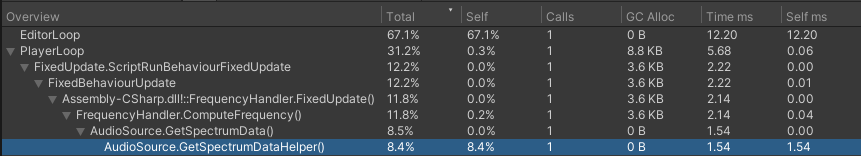
\includegraphics[width=0.75\textwidth]{profiler_spectrum.png}
    \caption{Profileranalyse für GetSpectrumData}
    \label{sec:profiler_spectrum}
\end{figure}
Eine Verzögerung von 1.5ms durch die eigentliche Berechnung erzeugt keine Verzögerung, welche nichtmehr als echtzeit definiert werden kann, weshalb ich mich von hier an auf diesen Ansatz konzentrierte und weiter an der Tonerkennung arbeitete. Das Ziel eines Pitch Detection Algorithmus ist es, die Grundfrequenz (\ref{sec:Grundfrequenz}) eines Tons zu bestimmen. Da die Grundfrequenz nicht immer die stärkste Frequenz im Spektrum des Tons ist, stellt diese Aufgabe eine besondere Herausforderung dar. Es ist Ziel die Grundfrequenz möglichst genau zu bestimmen, ohne eine große Menge an Rechenleistung zu verbrauchen. \\
Da das Ziel war, den Algorithmus im Rahmen der Möglichkeiten von Unity zu entwickeln, entschied ich mich dazu einen eigenen Algorithmus zu konzipieren, welcher vorallem die Funktion GetSpectrumData von Unity so gut wie möglich einbindet. Der erste Schritt ist immer, zunächst die Daten vom Mikrofon mithilfe von GetSpectrumData als Spektrum zu erhalten. Die Funktion GetSpectrumData benötigt drei Parameter, wovon zwei direkten Einfluss auf den Algorithmus nehmen. Der erste wichtige Parameter ist ein Array, welches mit den Daten der FFT gefüllt werden soll. Die Länge des Array muss hierbei eine Potenz von 2 sein und darf die Länge von 8192 Feldern nicht überschreiten. Diese Limitierung führt auf die FFT zurück, welche eine Fensterfunktion anwendet um mögliche Informationsverluste zu verhindern, welche durch eine falsch \glqq abgeschnittene'' Periode zustande kommen. Eine Datensatzlänge in der Größe einer Potenz von 2 soll dieses Problem verhindern (\ref{sec:Fouriertransformation}).  So kommen wir auch direkt zu dem zweiten Parameter von GetSpectrumData nämlich der anzuwendenden Fensterfunktion. Es werden als Fensterfunktionen bereitgestellt: Rectangular, Triangle, Hamming, Hanning, Blackman und BlackmanHarris. Diese unterscheiden sich in der Komplexität und dadurch auch in der Genauigkeit. In dem obigen Ausschnitt des Profilers sieht man GetSpectrumData mit der maximalen Arraygröße und der komplexesten Fensterfunktion. Die Entscheidung liegt hier also auf der besten Qualität der Berechnung, da selbst diese Rechenzeit noch weit im Rahmen von <= 30ms (\ref{sec:profiler_spectrum}) liegt \cite{lago2004quest}. Jetzt wo sich also das Spektrum relativ genau und schnell berechnen lässt gilt es noch den Rest der Tonerkennung darauf aufzubauen. Für die Konzeption des Algorithmus habe ich einige Ansätze aus den oben genannten Algorithmen analysiert und auf meine Verwendung angepasst. Ich habe zunächst das Spektrum in Obertöne bzw. den Grundton und Rauschen aufgeteilt. Die Obertöne bleiben dabei unverändert und das Rauschen setze ich auf null mithilfe eines einfachen Filters. Der Filter berechnet den Durchschnitt über das gesamte Spektrum und setzt alle Werte, die niedriger sind als dieser auf null. Da der Grundton ein relatives Maximum innerhalb des Spektrums ist, sollte dieser in den meisten Fällen nicht unter den Durchschnitt fallen. Der Grundton einer menschlichen Stimme 
schwingt bei jedem Menschen verschieden stark. Das ist vorallem der Fall bei tiefen, rauen Stimmen, weshalb ein Parameter eingeführt werden muss, welcher die Schwelle des Tonfilters regulieren kann. Einen ähnlichen Ansatz verfolgt der FDT Algorithmus, welcher ein sogenanntes \glqq Ruggedness spectrum'' aus Tälern und Bergen erzeugt, indem für jeden Datenpunkt eine Schwelle berechnet wird und daran entschieden wird, ob dieser in einem Tal oder auf einem Berg liegt. Die Schwelle wird nicht als Durchschnitt über den gesamten Datensatz, sondern nur über einen Ausschnitt rund um den zu untersuchenden Datenpunkt berechnet. Der Ansatz des FDT Algorithmus verbraucht dafür mehr Rechenzeit, denn es muss über jeden Datenpunkt iteriert werden und dann jeweils nocheinmal über die umliegenden Datensätze. Der hier vorgestelle Ansatz hingegen berechnet eine Konstante für alle Datenpunkte, indem einmal über alle Punkte iteriert wird und anschließend jeder Punkt entsprechen angepasst wird. \\
Die Datenpunkte sind jetzt gefiltert und müssen nur noch abgetastet werden um das letzte relative Maximum zu finden. Der Algorithmus geht zunächst davon aus, dass das absolute Maximum auch die Grundfrequenz ist, es werden zur Überprüfung alle früheren Datenpunkte untersucht, ob noch ein relatives Maximum auftritt. Existiert ein Maximum mit einem niedrigeren Index, so wird dieser Punkt als neue Grundfrequenz festgehalten. Um falsche Ausschläge trotz des Rauschfilters zu verhindern, darf die mögliche Grundfrequenz nur um einen bestimmten Prozentsatz vom absoluten Maximum abweichen. Dieses Tool wird dem Nutzer zur Anpassung an die Hand gelegt, falls der Grundton kaum von dem Rauschen abweicht. In diesem Fall ist der Rauschfilter zu extrem, da dieser den Grundton auch filtern würde. In diesem Fall bietet sich eine nicht so radikale Lösung an, in Form des prozentualen Abstands zum absoluten Maximum. Dieser Ansatz ist möglich, da die menschliche Stimme auf verschiedenen Tonhöhen größtenteils die gleichen Anteile an Obertönen erzeugt, sodass sich dieser prozentuale Unterschied kaum verändert. Über diese Eigenschaft lässt sich auch die zu einem großen Teil immer gleich klingende Stimmfarbe eines Menschen erklären, da die Obertöne diese ausmachen. Die einzige Ausnahme hierbei ist, wenn der Mensch aktiv versucht die Stimmfarbe zu verändern. \\
Aktuell kann der Algorithmus nur den Index des gefundenen Grundtons zurückgeben, ich brauche allerdings die Frequenz. Um die Frequenz aus dem Index zu berechnen, benötige ich einen Wert, welcher angibt, wie viel Hz pro Schritt im Array gegangen werden. Dieser Koeffizient lässt sich berechnen aus der Samplerate des Mikrofons geteilt durch zwei, umso die maximale abtastbare Frequenz zu erhalten (\ref{sec:Abtast}). Dieser Wert muss noch verteilt auf alle Werte des Spektrums betrachtet werden.
Es sei $s_{mic}$ die Samplerate des Mikrofons und $\bar{x}$ die Anzahl der Werte des Spektrums, so können wir den Koeffizienten $F_c$ wie folgt berechnen.
$$ F_c = \frac{s_{mic}}{2\bar{x}} $$
Es ist einfach von dem Index auf die Frequenz zu schließen, indem der Index mit dem Koeffizienten multipliziert wird. Die entstandene Abstufung der Frequenzen pro Index ist sehr ungenau, weshalb zuletzt noch zwischen den höchsten Werten interpoliert werden muss, um das tatsächliche Maximum annähernd bestimmen zu können und die Frequenz so genau wie möglich angegeben werden kann. Hierfür wende ich eine einfache Newton Interpolation auf die drei Punkte um den maximalen Wert des relativen Maximums. Die Rechenleistung wird so reduziert, da das Maximum innerhalb dieser drei Werte liegen muss. 

%TODO gehört in Implementierung
\begin{algorithm}
    \caption{Pitch Detection Algorithm} \label{pda}
   \begin{algorithmic}[1]
    \Require {filter, threshold, cutoff}
    \Function {ComputeFrequency}{}
        \State spectrum=GetSpectrumData()
        \State spectrumCut = first values of spectrum till cutoff Value 
        \State absMaxIndex = 0 
        \State max = maximum of spectrumCut
        \State avg = average of spectrumCut
        \For{$i = 1$ \textbf{to} length of spectrumCut $- 1$} 
            \If{spectrumCut[i] < avg $*$ filter} 
                \State spectrum[i] = 0
                \State \textbf{continue} to next iteration
            \EndIf
            \If{spectrumCut = max}
                \State absMaxIndex = i
            \EndIf
        \EndFor
        \State bestIndex = HandleOvertones(absMaxIndex)
        \State interpolatedIndex = Interpolate(bestIndex)
        \If{interpolatedIndex != 0}
            \State \textbf{return} interpolatedIndex $* \ F_c$
        \EndIf
        \State \textbf{return} bestIndex $* \ F_c$
   \EndFunction
    \State
    \Function{HandleOvertones}{absMaxIndex}
        %\Require absMaxIndex, spectrum\_cut
        \State overtoneMax = 0
        \State overtoneMaxIndex = absMaxIndex
        \For{i = absMaxIndex \textbf{to} 1}
            \State currentVal = spectrumCut
            \If{currentVal = 0}
                \State overtoneMax = 0
            \EndIf
            \If{currentVal > spectrumCut $*$ threshold}
                \If{overtoneMax < currentVal}
                    \State overtoneMax = currentVal
                    \State overtoneMaxIndex = i
                \EndIf
            \EndIf
        \EndFor
        \State \textbf{return} overtoneMaxIndex
    \EndFunction
    \end{algorithmic}
\end{algorithm}

\subsubsection*{Berechnung der Laufzeitkomplexität des vorgestellten Algorithmus}
Es gilt zu zeigen, dass der oben vorgestellte Pitch Detection Algorithmus effizient ist. Ich werde die Funktion \glqq HandleOvertones'' zunächst untersuchen, da diese von der Funktion \glqq ComputeFrequency'' aufgerufen wird. Man kann sehen, dass die Zeilen 25 und 26, sowie die Zeile 39 nur einmal pro Ablauf aufgerufen werden und daher vernachlässigbar sind. Sei n die Länge des Spektrums. Die Schleife wird im worst case Szenario $n$ mal und die Zeile 27 $n + 1$ durchlaufen. 
$$3 * \mathcal{O}(1) + 7 * \mathcal{O}(1) * \mathcal{O}(n) + \mathcal{O}(1) = \mathcal{O}(n) $$
Die Laufzeitkomplexität der Funktion beläuft sich demnach auf $\mathcal{O}(n)$. Die Komplexität der Funktion \glqq ComputeFrequency'' werde ich zunächst betrachten ohne auf die Funktionsaufrufe einzugehen. Die Schleife in dieser Funktion wird immer $n$ mal und die Zeile 7 $n + 1$ ausgeführt. Alle anderen Zeilen werden nur einmal ausgeführt, sodass auch hier eine Schranke von $\mathcal{O}(n)$ gesetzt werden kann. Die aufgerufenen Funktionen sind jedoch nicht so Laufzeiteffizient. Berücksichtigt man noch die Funktionsaufrufe, so stellt man schnell fest, dass die Laufzeitkomplexität höher ausfällt. Geht man davon aus, dass GetSpectrumData eine gewöhnliche rekursive FFT berechnet, so beläuft sich die Laufzeitkomplexität dieser auf $\mathcal{O}(n \log{n})$. Eine Newton Interpolation hat sogar eine maximale Laufzeitkomplexität von $\mathcal{O}(n^2)$, diese Laufzeitkomplexität begründet auch, warum nur drei Punkte interpoliert werden. Da die Anzahl der zu interpolierenden Punkte fest ist, werde ich die Laufzeitkomplexität der Interpolation als konstant annehmen. Die Komplexität der Max, Avg und Copy Funktionen sind ebenfalls linear.
$$\mathcal{O}(n \log{n}) + 4 * \mathcal{O}(n) + 5 * \mathcal{O}(1) + 5 * \mathcal{O}(1) * \mathcal{O}(n) = \mathcal{O}(n \log{n})$$
Den größten Einfluss auf die Zeitkomplexität nimmt die von Unity zur verfügung gestellte Funktion, sodass der Algorithmus nicht weiter optimiert werden kann, da diese Funktion essenziell ist.

\chapter{Konzeption eines spielerischen Trainingsprogramms zur Gehörbildung}

Im folgenden Kapitel möchte ich auf die Konzeption einer spielerischen Trainingssoftware zur Gehörbildung eingehen. Unter die Konzeption fällt dabei, wie die Anwendung aufgebaut sein soll, wie auf Systemsicht mit den Eingaben umgegangen werden soll und schließlich das Erarbeiten eines Evaluationskonzept.


\section{Konzeption des Spiels}
%- Grundkonzepte (geleitet / einführung in das Thema) und erweiterbare Module (level Basiert)
%    - Tutorial / Lernkapitel
%    - Endlosübungen zur Festigung
%    - Geführte Einführung in Benutzung?
%    - Flow
%
%- Basierend auf den Erkenntnissen aus Kapitel 2 -> Aus der Analyse muss klar werden, was wichtig ist
% - Design Pattern?
%In der folgenden Sektion wird das Design der vom User wahrnehmbaren Entscheidungen beschrieben und erläutert.
%\subsection*{Überblick}

Ich werde nun auf die allgemeine Struktur der Anwendung eingehen aus Sicht des Nutzers beschrieben. Es werden nun also nur von dem Nutzer sichtbare Designentscheidungen diskutiert. Auf die genaueren Inhalte der einzelnen Szenen innerhalb des Spiels, sowie auf die Grundideen des Programms, werde ich auch eingehen. Der Nutzer soll mithilfe der Anwendung effektiv das Erkennen und Reproduzieren von Intervallen üben. Zum Lernen sollen dem Nutzer zwei Möglichkeiten gegeben werden, entweder kann Er eine geführte Lektionen basierte Einführung in das Thema absolvieren, wo Ihm auch Hilfestellungen gegeben werden um das Intervall effektiv zu erkennen, oder Er kann endlos Intervalle bestimmen zur Wiederholung und Festigung der Fähigkeiten. Die Aufgaben werden hierbei natürich zufallsgeneriert, sodass dem Nutzer niemals die Aufgaben ausgehen. Das Zufallsgenerieren von Aufgaben ist nicht selbstverständlich, wie aus der Analyse der State of the Art Anwendungen klar wird, denn einige der Anwendungen erlauben nur das Beantworten von vordefinierten Aufgaben. Dem Nutzer soll außerdem die Möglichkeit gegeben werden diese Aufgaben über das Mikrofon in Form von Gesang zu beantworten. Aus der Analyse des State of the Art wird klar, dass diese Option so gut wie keine Anwendung bietet, obwohl sie den Lerneffekt deutlich verbessern kann. Weiterhin soll es dem Nutzer möglich sein die Aufgabe durch einen Klick in das Notensystem zu beantworten, sollte dieser nicht singen wollen. Diese alternative Eingabemethode halte ich für besser als einen Button mit der richtigen Lösung zu drücke, wie es einige der State of the Art Anwendungen umsetzen. Im Gegensatz zu der simplen Auswahl einer Lösung durch einen Button kann durch das Anklicken der Note im Notensystem weiterhin ein Gefühl für das Erkennen von Noten vermittelt werden. Idealerweise kann die Anwendung alle relevanten Aspekte der Gehörbildung abfragen, wie etwa Akkorde erkennen oder ein Melodiediktat zu stellen, das würde jedoch den Rahmen dieser Arbeit sprengen. Ein einfaches \glqq Authoringtool'' zum Erstellen von Aufgaben, für den Lektionen basierten Teil ist hierbei schon ein erster Ansatz, um eventuell Lehrern die Möglichkeit zu geben eigene Aufgabensätze zu konzipieren und diese einfach einzubinden. Dabei soll es möglich sein das geforderte Intervall zu definieren und dazu eine Aufgabenstellung, sowie den Grundton zu definieren. Es ist in dem Zusammenhang der Tonerkennung auch wichtig, dass diese auf die Stimme jedes Nutzers angepasst werden kann, sodass auch hierfür ein Optionenmenü mit entsprechenden Anweisungen zur Anpassung der einzelnen Regler wichtig ist. Will man den Nutzer singen lassen, so muss auch sicher gestellt werden, dass dieser in seiner bevorzugten Stimmlage singen kann. Auch für diese Anpassung muss eine Option vorhanden sein. Weitere Anpassungsmöglichkeiten auf ür die Aufgaben selbst, sollen dem Nutzer weitere Tool an die Hand geben um sich so gezielt wie möglich fortzubilden. So etwa soll es dem Nutzer außerdem möglich sein den Grundton entweder zufällig zu generieren oder auch fest einzustellen oder die Richtung des Intervalls anpassen können, also ob dieses nach oben oder nach unten vervollständigt werden soll. Diese Vielzahl an Einstellungen sollen es dem Nutzer nicht nur ermöglichen ein bestimmtes Themenfeld zu lernen, sondern auch damit dieser eine gewissen Kontrolle über die Schwierigkeit hat und somit immer genau richtig beansprucht wird. Aus der Analyse kann man zudem erkennen, dass es besonders für unerfahrenere Nutzer, sehr von Vorteil sein kann, wenn es einige Erklärungen zu den wichtigsten musikalischen Grundlagen direkt auf der Plattform zum Nachlesen gibt. 

\subsection{Hauptmenü}
Wird die Anwendung gestartet, gelangt man in das \textbf{Hauptmenü}. Von dem Hauptmenü aus kann man zu den Spielmodi \glqq Endlosspiel'' und \glqq Modulen'' navigieren, sowie zu den allgemeinen Einstellungen und zu dem Theoriebuch. Außerdem lässt sich die Anwendung von hier aus auch beenden. Es wird dem Nutzer zur Überprüfung außerdem angezeigt in welcher Tonlage die Aufgaben generiert werden, sollte er einen Spielmodus starten.

\subsection{Einstellungen}
In den \textbf{allgemeinen Einstellungen} wird dem Nutzer ein kurzer Text zu der Anpassung der Tonerkennung angezeigt, sowie ein Notensystem an welchem dieser die Tonerkennung ausprobieren kann und überprüfen kann, ob diese gut genug auf die eigene Stimme eingestellt ist. Das Anpassen der Tonerkennung soll mithilfe von zwei Slidern geschehen, welche jeweils die zwei Werte \glqq Threshold'' und \glqq Filter'' anpassen. Slider bieten die genauste Schrittweite bei der Anpassung und sind gleichzeitig einfach zu verstehen. Weiterhin gibt es in den allgemeinen Einstellungen Dropdown Menüs über welche man die Tonlage und das Eingabegerät ändern kann. Durch einen Button gelangt man zurück zum Hauptmenü.

\subsection{Theoriebuch}
Das \textbf{Theoriebuch} soll aus einer Navigierleiste links im Bildschirm und einem Contentfenster im restlichen Bereich bestehen. Die Navigierleiste beinhaltet mehrere Buttons mit den Themen als Label, welche den Content in dem restlichen Bereich des Fensters anpassen. Da diese Szene von drei verschiedenen Szenen aufgerufen wird, existiert außerdem ein Button, welcher die vorherige Szene wieder lädt. Die Infotexte zu den Themen werden aus einem Musiktheorie Buch übernommen und sollten somit die notwendige pädagogische Kompetenz aufweisen um die Inhalte gut genug zu vermitteln. \cite{abcmusik} 

\subsection{Endlosübung}
Das \textbf{Endlosübung} zeigt auf der unteren Häfte des Bildschirms ein Notensystem an, auf welchem nicht nur der Grundton gerendert werden soll, sondern auch die Antwort eingegeben bzw. angezeigt werden soll. Entscheidet sich der Nutzer dazu die Note singen zu wollen, so soll die erklingende Note automatisch im rechten Drittel des Notensystem in echtzeit erscheinen. Möchte der Nutzer jedoch die Note per Maus setzen, so wird die unter dem Cursor liegende Note erscheinen, bewegt sich der Cursor weiter soll die Note nicht mehr gerendert werden. Klickt der Nutzer auf eine Note mit einem Linksklick, so soll diese Note eingeloggt werden und auch keine anderen Noten mehr gerendert werden können. Möchte der Nutzer einen Halbton eingeben, muss dieser einen Toggle aktivieren, welcher die ausgewählte Note um einen Halbton verschiebt. Um die Aufgabe zu lösen, muss die richtige Antwort für eine bestimmte Zeit gesungen werden, um falsche Erkennungen zu reduzieren. Wurde die Aufgabe richtig beantwortet erscheint ein Feedbacktext im oberen rechten Bereich der Szene, welche dem Nutzer mitteilt, dass die Antwort richtig ist. Erscheint dieser Text nicht, so ist die Aufgabe auch noch nicht gelöst. Sobald die Aufgabe gelöst ist, kann der Nutzer selbst entscheiden, wann er die nächste Aufgabe beginnen möchte mithilfe eines Buttons. Der extra Schritt den Nutzer auf weiter klicken zu lassen, soll verhindern, dass noch der Ton gesungen wird der letzten Aufgabe und schon der nächste Grundton gleichzeitig abgespielt wird. Zu Beginn jeder Aufgabe erklingt der Grundton des Intervalls über das Standardausgabegerät des Nutzers. Über einen Button soll es möglich sein, diesen Grundton so oft wie möglich sich erneut anhören zu können. Es ist außerdem möglich das Theoriebuch aufzurufen über einen Button. Weiterhin soll es möglich sein ein Anpassungsmenü aufzurufen, in welchem der Nutzer zurück in das Hauptmenü navigieren kann und die aktuelle Aufgabe überspringen kann, sollte er das wünschen. Es soll in diesem Menü außerdem möglich sein die Eingabemethode zwischen Gesang und manueller Eingabe zu wechseln, sowie einen festen Grundton definieren und die Richtung des Intervalls bestimmen zu können. Das Anpassungsmenü soll sich durch einen Klick auf einen Button schließen lassen. 

\subsection{Modulübung}
Zuletzt soll der \textbf{modulbasierte Spielmodus} ähnlich wie das Endlosspiel ein großes Notensystem implementieren in der unteren Hälfte des Bildschirms, während in der oberen Häfte alle relevanten Informationen angezeigt werden. Der Unterschied zum Endlosspiel ist dabei, dass statt zufällig generierten Aufgaben vorher definierte Aufgaben gestellt werden. Die Aufgaben können dabei den Grundton, das Intervall und den Text anpassen um so eine möglichst flexible Aufgabenstellung zu erlauben. Es soll außerdem möglich sein reine Textpassagen anzuzeigen, ohne eine Aufgabe zu stellen. Neben diesen Änderungen verglichen mit dem Endlosspiel, soll auch der modulbasierte Spielmodus ein Anpassungsmenü haben und auch eine Möglichkeit bieten die Theorie aufzurufen. Sind alle definierten Aufgaben abgeschlossen soll der Nutzer mit einem Klick auf \glqq Nächste Übung'' wieder in das Hauptmenü gelangen. 

\section{Konzeption der Systemkomponenten}
% Wie werden GUI Anfragen versendet, welches Modul erzeugt Töne, Aufgaben etc.
% Systemsicht: I/O Verarbeitung, Gui wie wird interagiert
%Eigene Gedanken und Ansätze müssen in Konzeption, Gründe dafür in Analyse

% 1. Tonerkennung
% 2. I/O
% 3. Aufgabengen
% 4. Datenstrukturen
%

Ich werde nun auf die Konzeption der Systemkomponenten eingehen und erläutern wie diese miteinander kommunizieren und interagieren sollen. Ich habe die Komponenten in vier Bereiche aufgeteilt, welche aus der Tonerkennung, dem Input und Output handling, der Aufgabenerzeugung und den Datenstrukturen bestehen.\\
\subsection{Tonerkennung}

Die \textbf{Tonerkennung} soll aus zwei Klassen zusammengesetzt sein. Der FrequencyReader soll das Mikrofon initialisieren, die Daten aus dem Mikrofon auslesen und schließlich der zweiten Klasse dem FrequencyHandler zur Verfügung stellen. Das Initialisieren soll dabei nicht nur das Mikrofon starten, sondern auch die erwähnten Maßnahmen (\ref{sec:analyse_echtzeit}) umsetzen, damit das Auslesen in Echtzeit geschehen kann. FrequencyReader stellt die Mikrofondaten und die zum Aufnehmen verwendete Samplerate bereit. FrequencyHandler greift auf die bereitsgestellten Daten von FrequencyReader zu um den vorgestellten Pitch Detection Algorithmus (\ref{pda}) auf die eingelesenen Daten des Mikrofons anzuwenden. Auf die Samplerate muss FrequencyHandler ebenfalls zugreifen um $F_c$ berechnen zu können (\ref{sec:analyse_echtzeit}). Der Pitch Detection Algorithmus muss jeden Frame neu ausgeführt werden, um die neuen Mikrofondaten zu analysieren. FrequencyHandler stellt die Frequenz und den Namen der dazugehörigen Note anderen Klassen bereit.\\

\subsection{Input / Output}
Die \textbf{Eingabe und Ausgabe} der Noten arbeitet eng mit der Tonerkennung zusammen, da die erkannten Töne in Echtzeit auf dem Bildschirm in einem Notensystem angezeigt werden sollen. Das Notensystem wird dabei sowohl als Eingabe, als auch als Ausgabe verwendet. Das Notensystem soll auf der linken Hälfte nur ermöglichen den Grundton zu rendern und auf der rechten Hälfte wahlweise entweder den vom Mikrofon eingelesenen Ton zu rendern oder die Auswahl des Nutzers beim darüber hovern mit dem Cursor zu rendern. Dementsprechend muss es also möglich sein die rechte Hälfte entweder als Output für das Mikrofon zu verwenden (Outputmode) oder als Input für den User (Inputmode). Im Inputmode muss weiterhin die Möglichkeit existieren Halbtöne auswählen zu können, welche auf der gleichen Höhe liegen wie der dazugehörige Ganzton. Es muss einen Parameter geben, welcher angibt ob der Ton, der gerendert werden soll, ein Halbton oder Ganzton ist. Das Notensystem muss in diesem Fall auch den Sprite des entsprechenden Ton anpassen können, sodass dieser das richtige Vorzeichen erhält. Es ist bei der Wahl des Vorzeichens wichtig, ob das Intervall nach oben oder unten vervollständigt wird, aufgrund der Beschaffenheiten wie Intervalle definiert sind \ref{sec:Intervalle}. Es muss also bei der Wahl des Vorzeichens auf den Parameter geachtet werden, welcher angibt, ob die Aufgabe ein nach oben oder unten generiertes Intervalle fordert. Das Notensystem soll weiterhin zu jedem möglichen Ton auf dem Notensystem ein Objekt besitzen, welches einige Sachverhalte vereinfachen soll. So hat jede dieser Noten eine Hitbox, welche auf dem Notensystem so angeordnet liegt, dass sie den dortigen Ton repräsentiert. Die Notenobjekte werden von dem Notensystem initialisiert mit ihrem entsprechenden Notenwert, sowie dem Wert des nächst tiefer und höher liegenden Halbtons. Da jede Note selbst überprüft, ob diese aktuell aktiv ist, müssen sie auch mit dem Notensystem kommunizieren können, um ein Signal senden zu können, falls eine Note mittels eines Linksklicks ausgewählt wurde. Ist das der Fall, sendet diese Note dem Notensystem ein Signal, dass diese ausgewählt wurde, woraufhin das Notensystem alle anderen Noten deaktiviert, bis die ausgewählte Note durch einen weiteren Linksklick deaktiviert wurde. Wird die Note wieder abgewählt, sendet die Note ebenfalls ein Signal an das Notensystem, sodass dieses alle anderen Noten wieder freigeben kann und diese wieder Wählbar sind. Das Notensystem weiß somit immer ob und welche Note aktiv ist und kann somit auf Anfrage den Wert der ausgewählten Note zur Verfügung stellen. Die Noten müssen außerdem Zugriff auf das Notensystem haben, um abfragen zu können, ob der Nutzer aktuell einen Halbton setzen möchte, damit diese entsprechend ihren Sprite anpassen können. Um zwischen dem Inputmode und Outputmode wechseln zu können müssen die Noten einen weiteren Parameter besitzen, welcher dem Notensystem erlaubt diese nicht mehr auf den Cursor des Nutzers reagieren zu lassen. Wird der Outputmode verwendet, so müssen die Noten über ihren Wert oder Namen angesprochen werden können. Es muss nun auch möglich sein mit dem Notensystem von außerhalb zu kommunizieren, damit nicht nur der aktuell gesungene Ton ausgegeben werden kann, sondern auch angepasste Töne. Das Notensystem benötigt schließlich noch die Möglichkeit ähnlich wie den Spielerton setzen zu können auch den linken Aufgabenton bzw. Grundton setzen zu können.\\
Damit der Input aus dem Mikrofon und der Input aus dem Notensystem gebündelt an einer Schnittstelle zugreifbar sind, werden diese von einem InputHandler mehrmals pro Frame abgerufen. Es wird so ein gewisses Maß an Abgrenzung zwischen Spiellogik und Input erreicht. Für die Ausgaben von Aufgabenstellung und Feedback soll eine allgemeine GameUI Klasse zuständig sein, damit auch dieser Output abgekapselt von der Spiellogik stattfindet und man somit einzelne Teile der Logik besser austauschen kann. \\
Die Generierung des Grundtons soll eine weitere Klasse übernehmen, welche einen Sinuston berechnet und diesen in eine AudioSource einbindet und schließlich auch direkt abspielt. Dadurch, dass die Klasse den Ton direkt in eine AudioSource einbindet, kann diese ganz einfach durch einen Button erneut abgespielt werden, ohne den Ton neu berechnen zu müssen.\\

\subsection{Gamelogic}
Die \textbf{Spiellogik} wird allgemein durch einen Elternklasse implementiert, sodass das Endlosspiel und der modulbasierte Übungsmodus von dieser Klasse erben können. Die grundsätzliche Kommunikation mit anderen Klassen bleibt bei beiden Klassen gleich, jedoch ist die Generierung eine Unterschiedliche. So wird bei dem Endlosspiel auf einem wahlweise zufälligem Grundton ein zufälliges Intervall nach oben oder unten gebildet. Bei dem modulbasierten Übungsmodus jedoch müssen die Aufgaben über eine json Datei selbst definiert werden. Die Elternklasse der Spiellogik sollte die Schnittstellen zu anderen Klassen definieren, darunter fallen der InputHandler, dem TonGenerator und der GameUI. Die Spiellogik soll alle Anpassungen vornehmen, welche den Spielverlauf verändern. Unter diese Entscheidungen fallen das Setzen eines festen Grundtons vom Nutzer, die Richtung der Intervalle und bei verändertem Input die entsprechenden Daten aus dem InputHandler zu verwenden. Außerdem soll die Spiellogik für die Generierung und Überprüfung der Aufgaben zuständig sein. \\

\subsection{Datenstruktur und Utility Klassen}
Schließlich müssen noch einige \textbf{Hilfsklassen und eine Datenstruktur} für Noten und Intervalle implementiert werden. Die Datenstruktur soll vorallem Noten und Intervale von ihren Namen auf eine Frequenz bzw. ein Frequenzverhältnis in Cent in der Gleichstufigen Stimmung definieren. Weiterhin werden in der Datenstruktur die Definitionen der Stimmlagen festgehalten, um schnell auf diese zugreifen zu können, mit entsprechenden Hilfsfunktionen, welche alle Lagen zurückgeben oder alle Töne innerhalb einer Lage. Es wird zusätzlich das Format zur Speicherung der Aufgaben der modulbasierten Übung definiert, um diese in einer Json speichern und anpassen zu können.
Die Hilfsklasse FrequencyUtil soll allen Klassen, welche Berechnungen mit Frequenzen machen müssen einige Basisfunktionen zur Verfügung stellen, welche die Berechnung auslagern. Es sollen Funktionen zur Berechnung eines Intervalls als Frequenzunterschied und zur Berechnung des daraus resultierenden zweiten Tons. Weiterhin werden Funktionen zur randomisierten Auswahl eines Grundtons und eines Intervalls aus der Datenstruktur zur Verfügung gestellt, sowie Hilfsfunktionen um den nächsten definierten Ton einer beliebigen Frequenz zu erhalten.

%TODO

\section{Evaluationskonzept}
%    - Hobby, Profi, Studierende
%    - Unterschiedliche Fragen für jede Gruppe? oder Unterschiedliche Wahrnehmung der Gruppen?
%    - Hobby
%        - Dazu gelernt? Hilfreich? Richtige Kompetenz oder zu schwer?
%    - Profi
%        - Soetwas gewünscht in der Ausbildung? Weiterhin praktisch zum fit bleiben? Empfehlung an Kollegen?
%    - Studierende  
%        - Richtige Ansätze für Uni? Hilfreich beim Lernen? Alle wichtigen Features dabei?
%    -allgemeine
%        - Wie war die Erkennung der Stimme
%        - Nutzbarkeit der Anwendungen
%       - Weiter verwenden?
    
Bei der Evaluation werde ich vorallem drei Gruppen meine Anwendung testen lassen und Sie dazu befragen. Diese drei Gruppen sind Hobbymusiker, professionelle Musiker und Musikstudenten. Dabei habe ich an jede Gruppe andere Ansprüche
und möchte auf die individuellen Bedürfnisse und Umstände dieser eingehen in der Evaluation. Daraus erhoffe ich mir ein möglichst komplettes Bild zu der Umsetzung der Trainingssoftware machen zu können und somit auch ein aussagekräftigeres Fazit ziehen zu können.
Ich habe die genannten Gruppen ausgewählt, da diese einen großen Teil der Musiker mit dem Blick auf das Wissen abdecken, aber auch unterschiedliche Instrumente und Musikarten abdecken können. Gerade die Studierenden sind interessant in Bezug auf die Lernwirkung, 
da diese im Studium das Modul Gehörbildung absolvieren müssen und sie daher einen besseren Bezug zu anderen Lernmethoden haben. \\
Ich möchte bei Hobbymusikern vorallem auf ihre vorhandene Motivation und neu erlangte Motivation durch das Trainingsprogramm eingehen. Außerdem möchte ich herausfinden, ob die vorrausgesetzten Kompetenzen zu viele waren und ob diese durch das Programm dennoch neu dazuerlangt werden konnten.
Ich gehe bei Hobbymusikern dabei am ehesten davon aus, dass diese noch nie oder nur im Instrumentalunterricht, sich mit Gehörbildung beschäftigt haben. Auf dieser Grundlage ist es für mich interessant ob 
das entwickelte Trainingsprogramm sie dazu anregen konnte sich etwas näher mit Gehörbildung auseinanderzusetzen und ob sie denken, dass sie in der Ausübung ihres Hobbys einen Mehrwerte daraus ziehen können. \\
Die Meinung der Studierenden ist vorallem wichtig in Bezug auf das Musikstudium und spezifisch auf Gehörbildung. Ich erhoffe mir von Studierenden den Nutzen für das Studium zu erfahren und was sie sich an einer solchen 
Anwendung noch zusätzlich wünschen würden. Außerdem möchte ich von Studierenden erfahren, ob die Anwendung das Wissen abfragt, welches von ihnen verlangt wird und sie dementsprechend lernen müssen.\\ 
Als letzte Gruppe möchte ich versuchen einige professionelle Musiker zu befragen. Deren Meinung ist besonders interessant, in Rückblick auf ihre Ausbildung, ob sie sich vorstellen könnten, dass ihnen eine solche Software in dieser Zeit
hätte geholfen. Außerdem wäre es interessant, ob sie sich vorstellen könnten so Gehörbildung weiterhin zu trainieren und ob sie diese Trainingssoftware ihren Kollegen weiter empfehlen würden.\\ 
Abschließend gibt es einige Aspekte zu erwähnen, welche alle der oben genannten Gruppen betreffen und sie dementsprechend alle beantworten können sollten. Unter diese Aspekte fallen die allgemeinen Punkte der Software, wie etwa die Performance oder die Zufriedenheit mit 
der Tonerkennung. Weiterhin fallen unter die allgemeinen Punkte, wie gut die Nutzer mit der generellen Handhabung der Software zurecht kamen und ob sie die Software planen weiter zu verwenden.
Weiterhin ist es wichtig grobe Angaben zu der verwendeten Hardware zu erhalten, falls die Tonerkennung nicht wie gewünscht funktioniert hat lassen sich so hoffentlich Zusammenhänge zu nicht optimaler Hardware herstellen.

\chapter{Prototypische Realisierung in Unity3D}

%- Töne u. Intervalle vorspielen; Erkennung / Einordnung von Tönen
%- Intervalle ergänzen, selbst singen u. dessen Verarbeitung
%- Adäquate GUI mit Feedback
%- Wie wurde das eingebundene realisiert
%- Warum Unity und kein andere Engine
%- Typisches Ergebnis ist UML Diagram
%- Laufzeitanalyse (wegen echtzeit aspekt)
% GUI einbinden als bild
\section{Implementierung des UI}

\section{Implementierung der Systemkomponenten}
Im folgendenen wird die Entwicklung der protypischen Trainingssoftware zur Gehörbildung näher beleuchtet und der Prozess der Umsetzung der Konzeption gezeigt. Ich werde die konzipierten Systemkomponenten alle einzeln ansprechen und wie diese umgesetzt wurden. 

In Unity gibt es die sogenannte MonoBehaviour Superklasse, welche einige Funktionen implementiert welche die Unity - Engine zu bestimmten Zeiten aufruft, wenn ein Skript, welches von MonoBehaviour erbt, in einer Szene eingebunden ist. Zu den wichtigsten Funktionen zählen die Funktion Start() und Update(). Start wird automatisch einmal während der Initialisierung des Skripts aufgerufen, wohingegen Update jeden Frame genau einmal aufgerufen wird. Es existieren noch weitere dieser Funktionen, wie etwa die Funktion FixedUpdate(), welche unabhängig von der Framerate in einem fixen Zeitintervall aufgerufen wird.

\subsection*{Tonerkennung}

Die Tonerkennung wurde realisiert mithilfe von zwei Klassen, welche von MonoBehaviour erben und jeweils ein eigenes GameObject in der Spielszene darstellen, sowie einer AudioSource, welche ebenfalls als alleinstehendes GameObject in der Szene existiert. Wie bereits konzipiert ist eine der Klassen (FrequencyReader) zuständig dafür das Mikrofon zu initialisieren, wohingegen die andere Klasse (FrequencyHandler) die tatsächliche Tonerkennung durchführt. \\
FrequencyReader implementiert ein öffentliches Attribut \glqq playback'', welches die AudioSource mit den geladenen Mikrofondaten repräsentiert und eine Konstante \glqq SampleRate'', welche die Samplerate von 44100Hz festlegt und freigibt. Die Klasse implementiert nur die Funktion Start(). Es werden in Start() das gewählte Eingabegerät aus dem SceneHandler abgerufen und daraufhin der AudioClip von playback direkt gesetzt. Es muss dann noch der Parameter loop der AudioSource playback auf true gesetzt werden. Dieser Parameter ermöglicht es dass die AudioSource den festgelegten Clip unendlich oft wiederholt und nicht nach einem Durchlauf abbricht. Es muss abschließend noch die Position der Daten des Mikrofons noch solange gepolled werden, bis Daten eingelesen werden, und die AudioSource abgespielt werden. 

\chapter{Evaluation / Validierung der erarbeiteten Methoden und Konzepte}

%- Mehrstufige Validierung mit Musikverein, Studenten, ...
%- Unterschiedliche Validierungen vergleichen
%- Konzept in 3 Stufen
%-- Vorbereitung, Durchführung, Nachbereitung
%-> Wie gemacht: Was will ich messen(ERkennungsrate, UX Bewertung)
% Auf quintessenz eingehen, gesamte Eval. in den Anhang
% nenne samplegröße, durchschnittsalter, frau/mann zusammensetzung

\section{Vorbereitung}
\section{Durchführung}
\section{Auswertung}


\chapter{Zusammenfassung}

%- Zusammenfassung
%- Ausblick
%-- Offene Fragen? (Real time Erkennung, ...)
%--- Umsetzung für Chor? Machine Learning zur Unterscheidung? AI Dirigent?
%Literaturverzeichnis (APA)

